\def\BackBleedLeft{209.594}\def\BackGridStart{245.594}
\def\BackContentLeft{251}\def\BackRuleRight{385}
\def\PhotoRight{359}\def\PhotoCenter{305}\def\BioLeft{379}
\def\BarcodeLeft{681.730}
\def\BarcodeGraphic{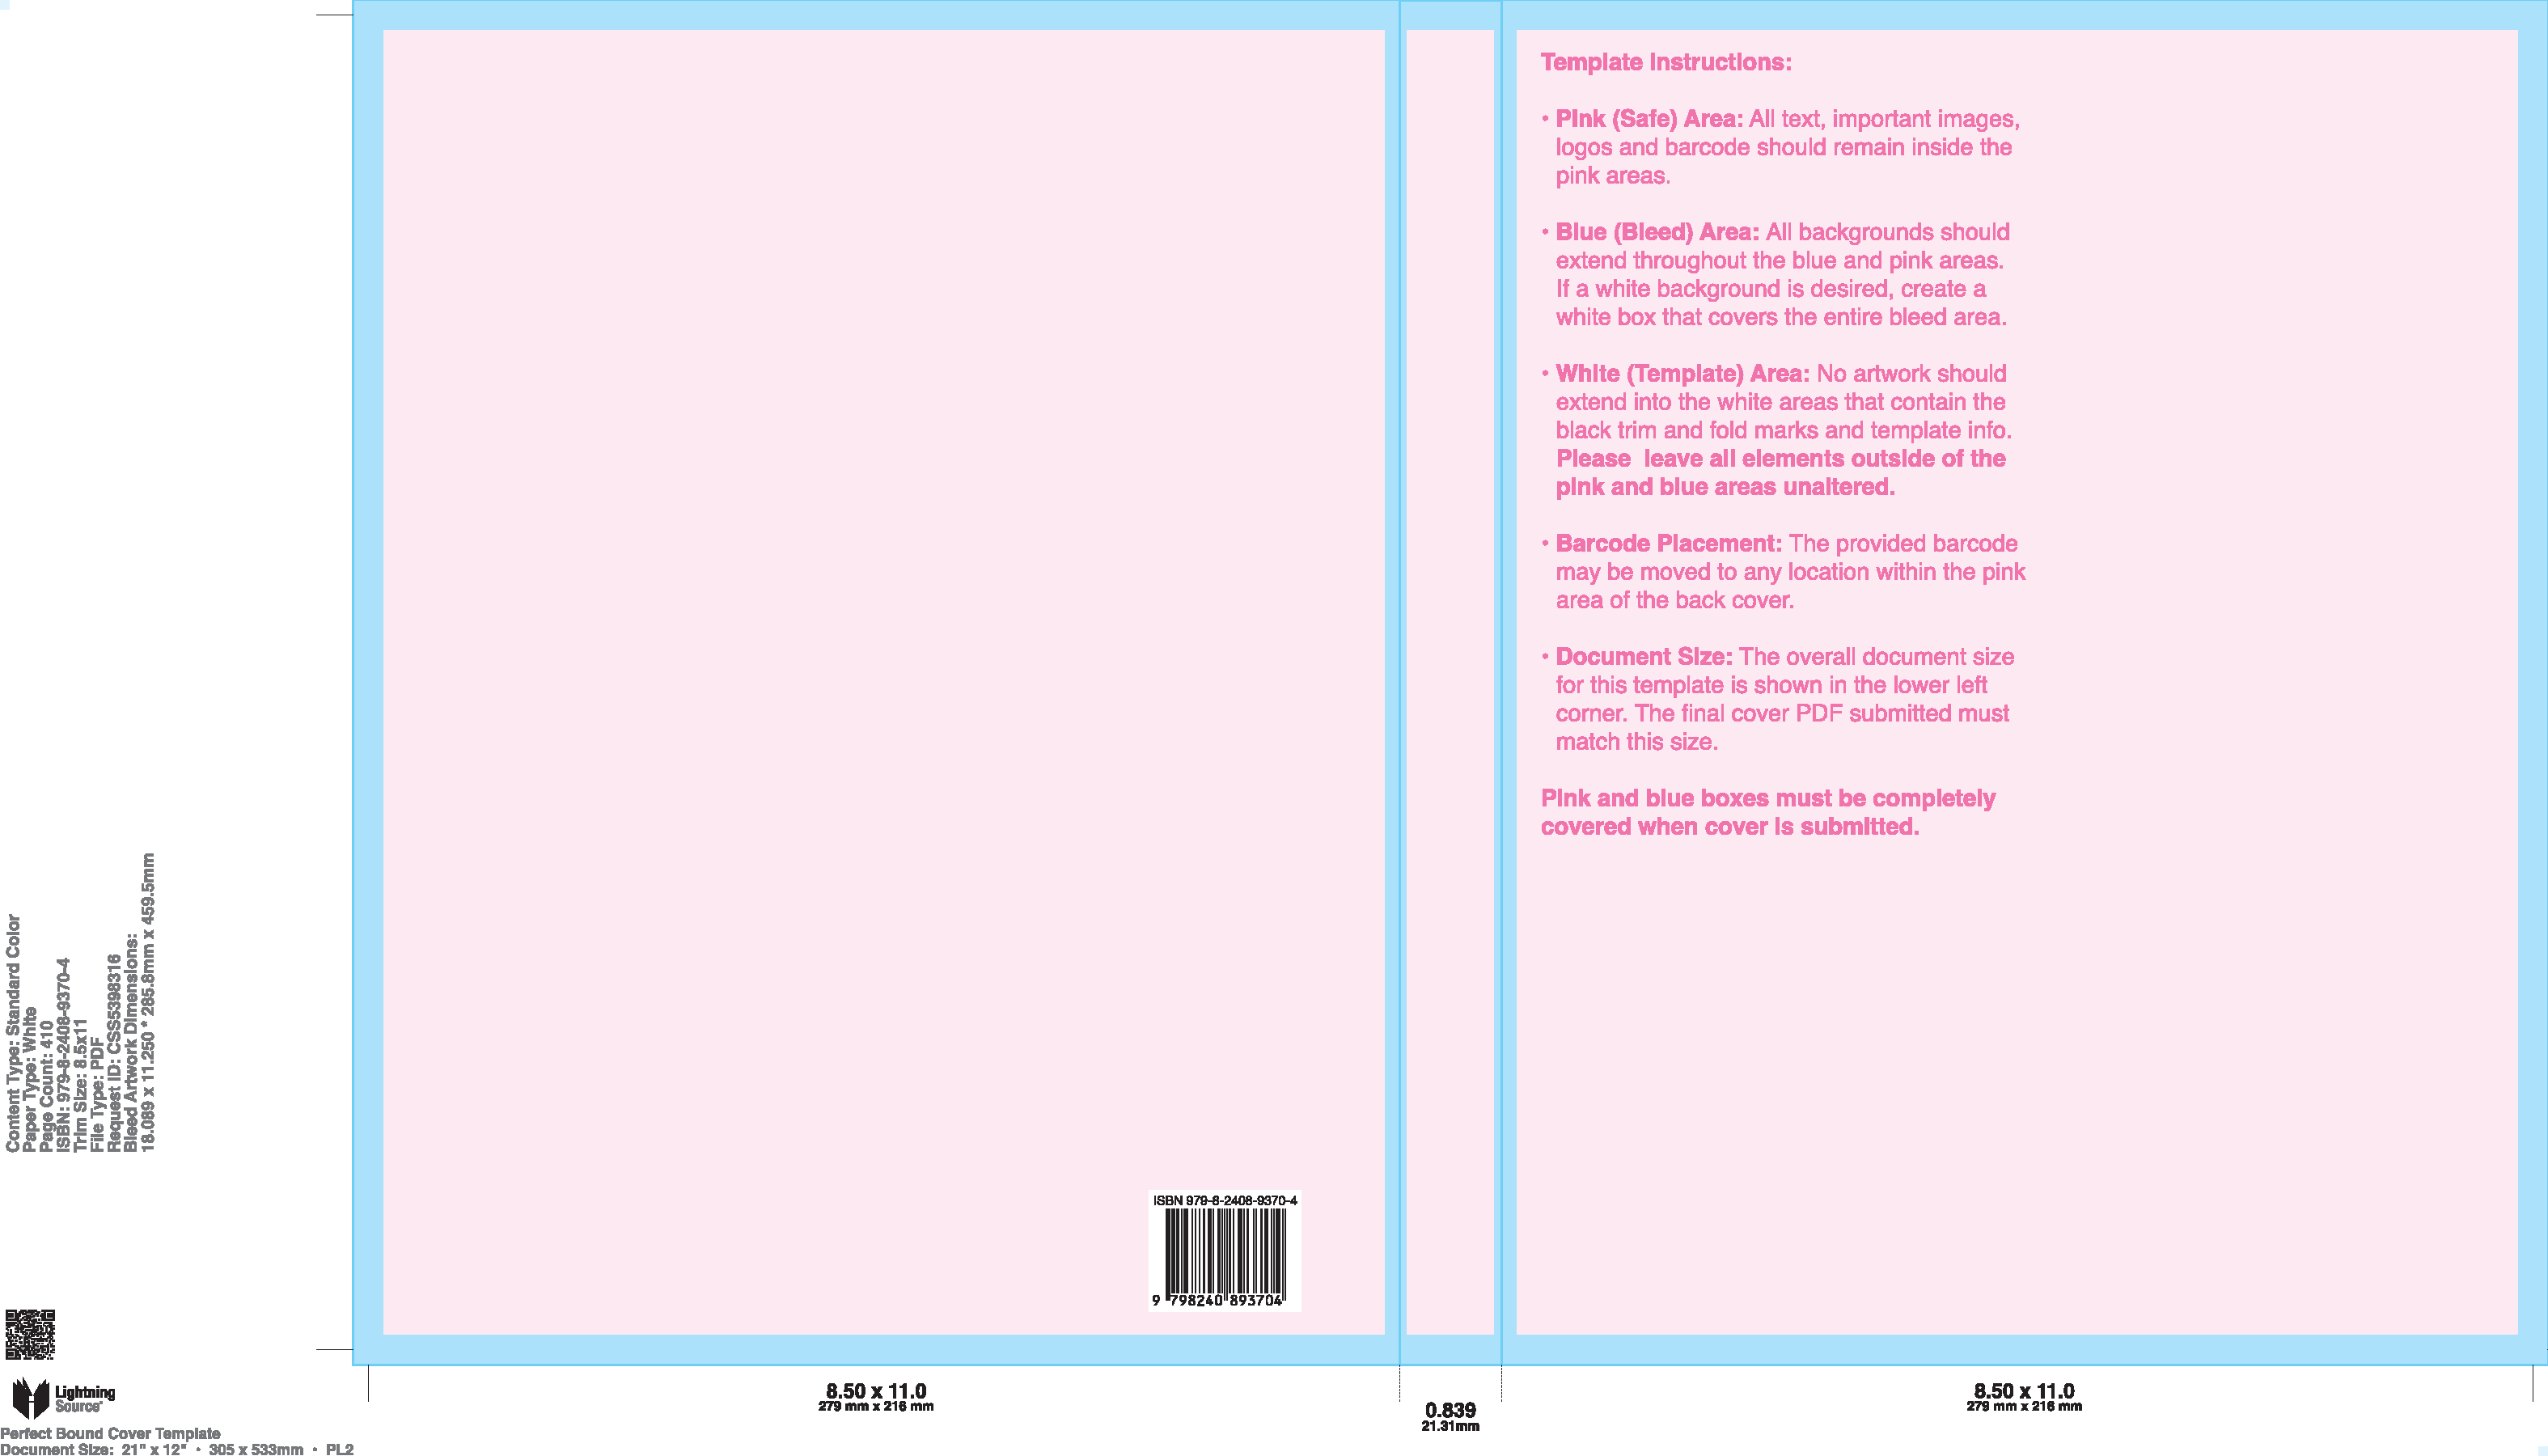
\includegraphics[viewport=681.730 85.695 772.094 157.695,clip,width=90.364pt,height=72pt]{../../templates/9798240893704-Perfect.pdf}}
\def\SpineCenter{860.775}\def\SpineTitleSize{8.15}\def\SpineLeading{9.3}
\def\SpineTitle{SOFTWARE DELIVERY, OPERATIONS, AND EVOLUTION}
\def\VolumeLabel{VOLUME II}\def\Accent{redaccent}
\def\TitleSize{34}\def\TitleLeading{38}\def\TitleRuleY{510}\def\EditionY{486}
\def\FrontTitle{Software Delivery,\par Operations, and Evolution}
\def\BackHeadline{Move software confidently through production.}
\def\BackCopy{Software Delivery, Operations, and Evolution examines what happens after software moves toward production: how systems are integrated, delivered, deployed, secured, operated, maintained, and improved over time.\\[7pt]
The book covers CI/CD pipelines, relational and NoSQL data systems, REST and GraphQL APIs, Docker, Kubernetes, serverless computing, infrastructure as code, cloud deployment, software security, incident response, technical debt, refactoring, legacy systems, maintenance, professional practice, and lifecycle integration.\\[7pt]
Practical examples, terminal demonstrations, diagrams, exercises, and project-based applications connect modern delivery and operations concepts with real-world software engineering.\\[7pt]
Designed for students, instructors, software engineers, DevOps practitioners, cloud professionals, and technical leaders, Volume II provides a practical guide to operating and evolving dependable production software.}
\def\CoverMotif{\begin{scope}[shift={(980,230)},scale=.86,draw=cyan,line width=1.5pt]
\draw[rounded corners=18pt](0,90)--(75,90)--(115,145)--(200,145)--(245,90)--(330,90)--(375,35)--(455,35);\draw[redaccent,line width=2.4pt,->](455,35)arc(-90:255:82);
\foreach \x/\y/\n in {0/90/BUILD,115/145/INTEGRATE,245/90/DELIVER,375/35/OPERATE,455/117/EVOLVE}{\fill[navy2,draw=cyan](\x,\y)circle(18pt);\node[text=ice,font=\fontsize{6.3}{7.4}\selectfont]at(\x,\y){\n};}
\foreach \x/\y in {75/90,200/145,330/90,455/35}\fill[redaccent](\x,\y)circle(4pt);\draw[redaccent,line width=1pt](115,115)rectangle(195,62);\draw[cyan,line width=.7pt](125,104)--(185,104)(125,92)--(175,92)(125,80)--(181,80);\end{scope}}
\documentclass{article}
\usepackage[paperwidth=21in,paperheight=12in,margin=0in]{geometry}
\usepackage{graphicx,tikz,xcolor,fontspec}
\usetikzlibrary{calc}
\pagestyle{empty}
\setmainfont{TeX Gyre Heros}
\definecolor{navy}{cmyk}{1,0.82,0.32,0.68}
\definecolor{navy2}{cmyk}{0.96,0.76,0.28,0.55}
\definecolor{blue}{cmyk}{0.92,0.67,0,0.10}
\definecolor{cyan}{cmyk}{0.72,0.02,0,0}
\definecolor{ice}{cmyk}{0.10,0.02,0,0}
\definecolor{white}{cmyk}{0,0,0,0}
\definecolor{redaccent}{cmyk}{0.08,0.92,0.62,0.20}
\begin{document}
\noindent\begin{tikzpicture}[remember picture,overlay,x=1pt,y=1pt]
\begin{scope}[shift={(current page.south west)}]
  % Full official bleed rectangles; coordinates come from the supplied template.
  \fill[navy] (\BackBleedLeft,54.0977) rectangle (825.406,864);
  \fill[navy2] (825.386,54.0977) rectangle (890.980,864);
  \fill[navy] (891,54.0977) rectangle (1512,864);
  \begin{scope}[opacity=.10]
    \foreach \x in {\BackBleedLeft,\BackGridStart,...,1512} \draw[cyan,line width=.35pt] (\x,54.0977)--(\x,864);
    \foreach \y in {54.0977,90.0977,...,864} \draw[cyan,line width=.35pt] (\BackBleedLeft,\y)--(1512,\y);
  \end{scope}

  % Back cover: all foreground objects are conservatively inset from the safe box.
  \node[anchor=north west,text=cyan,font=\bfseries\fontsize{10}{12}\selectfont] at (\BackContentLeft,814)
    {THE COMPLETE SOFTWARE ENGINEERING LIFECYCLE · \VolumeLabel};
  \draw[\Accent,line width=3pt] (\BackContentLeft,790)--(\BackRuleRight,790);
  \node[anchor=north west,text=white,text width=516pt,align=left,font=\bfseries\fontsize{19}{23}\selectfont] at (\BackContentLeft,766)
    {\BackHeadline};
  \node[anchor=north west,text=ice,text width=516pt,align=left,font=\fontsize{10.3}{14.1}\selectfont] at (\BackContentLeft,704)
    {\BackCopy};

  \node[anchor=north west,text=cyan,font=\bfseries\fontsize{9.3}{11}\selectfont] at (\BackContentLeft,372) {ABOUT THE AUTHOR};
  \begin{scope}
    \clip[rounded corners=4pt] (\BackContentLeft,246) rectangle (\PhotoRight,354);
    \node[anchor=center,inner sep=0] at (\PhotoCenter,300)
      {
\includegraphics[width=155pt]{../../cover/assets/moody-amakobe-cmyk.jpg}};
  \end{scope}
  \draw[cyan,line width=.8pt,rounded corners=4pt] (\BackContentLeft,246) rectangle (\PhotoRight,354);
  \node[anchor=north west,text=white,font=\bfseries\fontsize{12}{14}\selectfont] at (\BioLeft,352) {Moody Amakobe};
  \node[anchor=north west,text=ice,text width=350pt,align=left,font=\fontsize{8.15}{10.6}\selectfont] at (\BioLeft,329)
    {Moody Amakobe is an academic, applied researcher, and technology professional with extensive experience in software engineering, systems architecture, artificial intelligence, and graduate computing education. He holds a Doctor of Computer Science from Colorado Technical University and has held senior engineering and architecture roles with T-Mobile, Accenture, Wipro, and Deloitte. His teaching and research focus on connecting rigorous computing concepts with real-world engineering practice.};
  \node[anchor=south west,text=cyan,font=\bfseries\fontsize{8.4}{10}\selectfont] at (\BackContentLeft,206)
    {OPEN EDUCATIONAL RESOURCE · CC BY 4.0};
  \node[anchor=south west,text=ice,font=\fontsize{8.4}{10}\selectfont] at (\BackContentLeft,184)
    {GLOBAL DATA SCIENCE INSTITUTE};

  % Preserve the supplied ISBN-specific barcode as vector content at its official location.
  \node[anchor=south west,inner sep=0] at (\BarcodeLeft,85.695) {\BarcodeGraphic};

  % Spine: centered in the official pink safe spine region.
  \node[rotate=90,text=white,font=\bfseries\fontsize{\SpineTitleSize}{\SpineLeading}\selectfont] at (\SpineCenter,482)
    {\SpineTitle};
  \node[rotate=90,text=cyan,font=\fontsize{8.1}{9.5}\selectfont] at (\SpineCenter,171) {MOODY AMAKOBE};

  % Front cover typography.
  \fill[\Accent] (930,789) rectangle (937,830);
  \node[anchor=north west,text=cyan,font=\bfseries\fontsize{9.7}{11.5}\selectfont] at (956,824)
    {THE COMPLETE SOFTWARE ENGINEERING LIFECYCLE · \VolumeLabel};
  \node[anchor=north west,text=white,text width=500pt,align=left,font=\bfseries\fontsize{\TitleSize}{\TitleLeading}\selectfont] at (956,756)
    {\FrontTitle};
  \draw[\Accent,line width=4pt] (956,\TitleRuleY)--(1128,\TitleRuleY);
  \node[anchor=north west,text=ice,font=\fontsize{11}{13}\selectfont] at (956,\EditionY) {2026 EDITION};

  % Distinct lifecycle abstraction supplied by each volume wrapper.
  \CoverMotif

  \node[anchor=south west,text=white,font=\bfseries\fontsize{19}{22}\selectfont] at (956,135) {Moody Amakobe};
  \node[anchor=south west,text=cyan,font=\fontsize{8.8}{10.5}\selectfont] at (956,105)
    {GLOBAL DATA SCIENCE INSTITUTE};
\end{scope}
\end{tikzpicture}\null
\end{document}

